\documentclass{article}
\usepackage{tikz, comment}
\usepackage{pifont}
\usepackage{fontspec}
\usetikzlibrary{arrows, decorations.markings, decorations.pathreplacing}
\begin{comment}
:Title: Not defined yet
:Tags: average rate of change, arc ;area between curves;area using parametric equations,parametric integral formula;approximation by differentials;arc length of a curve
:Prob: 0.4972;0.4688;0.4672;0.4671;0.4615
:Slug: No name yet

Description Here.........
\end{comment}
\begin{document}\centering

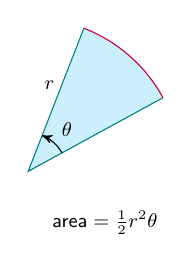
\begin{tikzpicture}[>=latex,xscale=.5*0.65, yscale=.5*0.65][font=\sf\small]

\draw[white, fill=cyan!20, samples=100, smooth, domain= 0.5:1.2, variable=\t]
plot ({6*cos(\t r)}, {6*sin(\t r)}) --(0, 0) ;
\draw[teal] ({6*cos(0.5 r)}, {6*sin(0.5 r)}) -- (0, 0) -- ({6*cos(1.2 r)}, {6*sin(1.2 r)}) node[black, left, pos=0.6, scale=0.8] {$r$};

\draw[purple, samples=100, smooth, domain= 0.5:1.2, variable=\t]
plot ({6*cos(\t r)}, {6*sin(\t r)}) ;

\draw[->, >=stealth', samples=100, smooth, domain= 0.5:1.2, variable=\t]
plot ({1.5*cos(\t r)}, {1.5*sin(\t r)});
\node[xshift=14, yshift=15, scale=0.8] at (0,0) {$\theta$};

\node[scale=0.8] at (3,-2) {$\hbox{area} = \frac{1}{2} r^2 \theta$};

\end{tikzpicture}\hskip1cm
\end{document}